\documentclass[12pt]{article}
\usepackage{graphicx}
\usepackage[none]{hyphenat}
\usepackage{graphicx}
\usepackage{listings}
\usepackage[english]{babel}
\usepackage{graphicx}
\usepackage{caption} 
\usepackage{booktabs}
\usepackage{array}
\usepackage{amssymb} % for \because
\usepackage{amsmath}   % for having text in math mode
\usepackage{extarrows} % for Row operations arrows
\usepackage{listings}
\lstset{
  frame=single,
  breaklines=true
}
\usepackage{hyperref}
  
%Following 2 lines were added to remove the blank page at the beginning
\usepackage{atbegshi}% http://ctan.org/pkg/atbegshi
\AtBeginDocument{\AtBeginShipoutNext{\AtBeginShipoutDiscard}}


%New macro definitions
\newcommand{\mydet}[1]{\ensuremath{\begin{vmatrix}#1\end{vmatrix}}}
\providecommand{\brak}[1]{\ensuremath{\left(#1\right)}}
\newcommand{\solution}{\noindent \textbf{Solution: }}
\newcommand{\myvec}[1]{\ensuremath{\begin{pmatrix}#1\end{pmatrix}}}
\providecommand{\norm}[1]{\left\lVert#1\right\rVert}
\providecommand{\abs}[1]{\left\vert#1\right\vert}
\let\vec\mathbf


\begin{document}

\begin{center}
\title{\textbf{VECTORS}}
\date{\vspace{-5ex}} %Not to print date automatically
\maketitle
\end{center}

\setcounter{page}{1}

\section{10$^{th}$ Maths - Chapter 10}

This is Problem-3 from Exercise 10.3

\begin{enumerate}
\item Find the projection of the vector $\hat{i}-\hat{j}$ on the vector $\hat{i}+\hat{j}$  
\end{enumerate}
\section{SOLUTION}
Given points are
\begin{align}
 \vec{A}=\myvec{1\\ -1} ,
 \vec{B}=\myvec{1\\ 1}
\end{align}

The formula of the projection vector :
 
\begin{align}
	\frac{\vec{A}^\top.\vec{B}}{\norm{\vec{B}}^2} \vec{B}
\end{align}

Find the projection vector $\vec{C}$ :
\begin{align}
	\vec{A}^\top \vec{B} = \myvec{1 &-1} \myvec{1\\ 1}=\myvec{1 *1}+\myvec{-1 * 1}=0
\end{align}

\begin{align}
	\norm {\vec {B}^2} = (\vec{B}^\top  \vec{B})=\myvec{1 & 1} \myvec{1\\ 1}= (1 * 1)+(1 * 1)=2
\end{align}

\begin{align}
\vec{C} = 
	\frac{\vec{A}^\top  \vec{B}}{\norm {\vec{B}}^2} \vec{B}
   =\frac{0}{2} \myvec{1\\ 1}
	=\myvec{0\\ 0}
\end{align}
\begin{align}
	\vec{C}=\myvec{0\\ 0}
\end{align}
\begin{figure}[h]
  \centering
  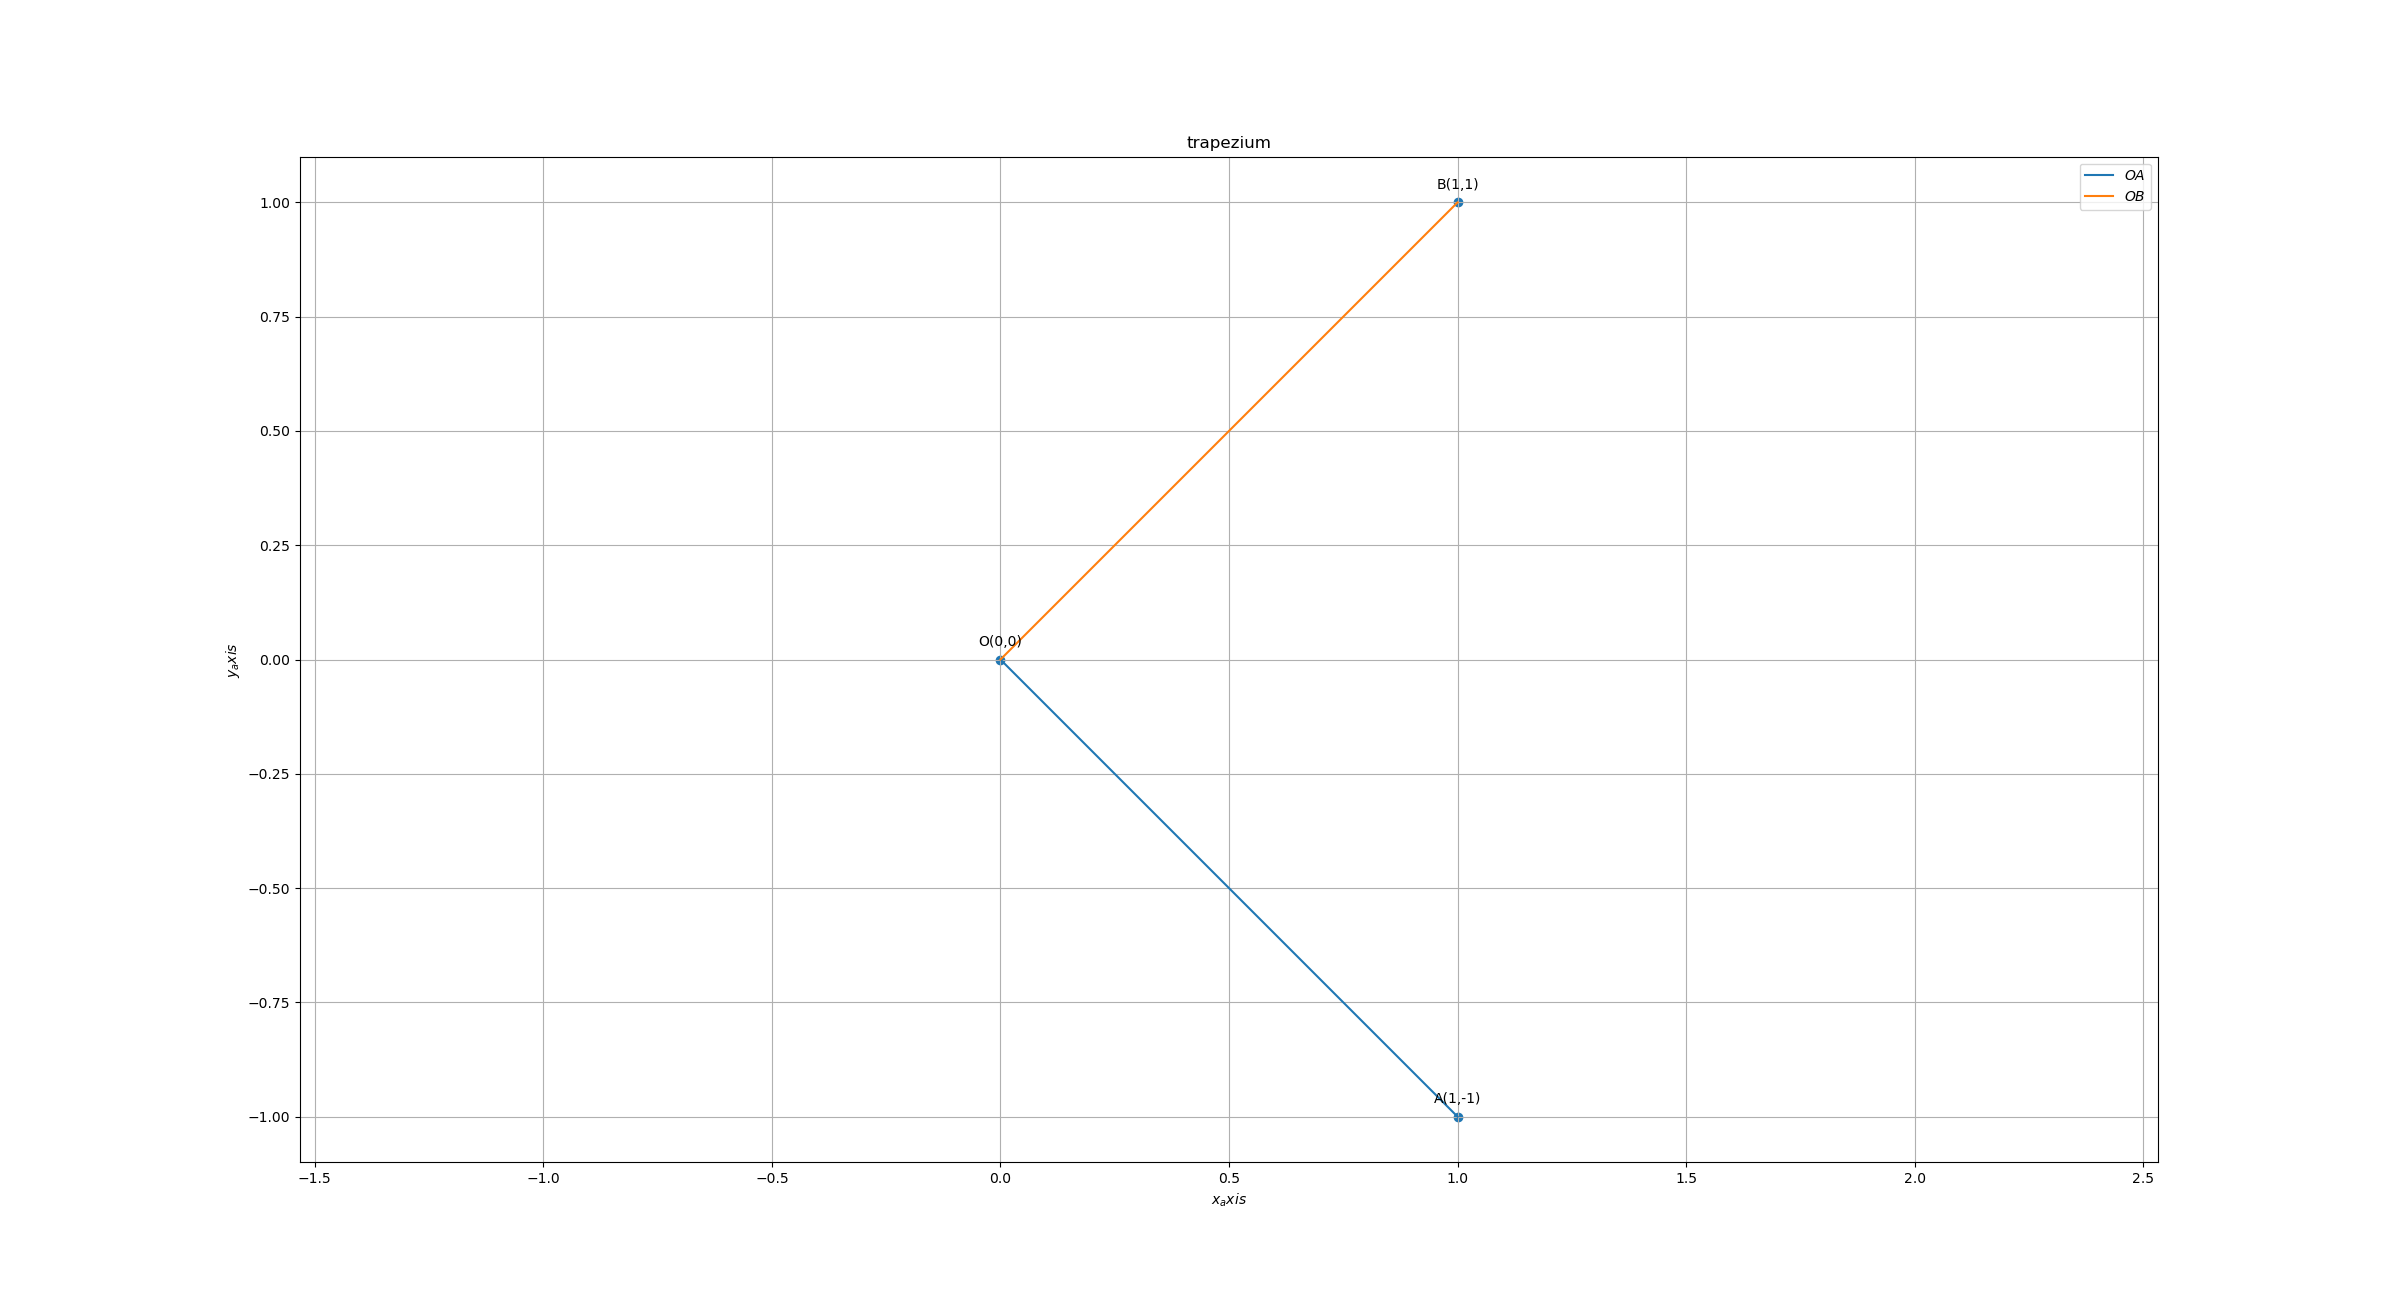
\includegraphics[width=\columnwidth]{vector.png}
\caption{}
\end{figure}

\end{document}
